% Generated from the Markdown write-up by scripts/render_drafter_learnings.py.
\documentclass[11pt,a4paper]{article}
\usepackage[margin=16mm]{geometry}
\usepackage[T1]{fontenc}
\usepackage[utf8]{inputenc}
\usepackage{lmodern,microtype,multicol,graphicx,xcolor}
\usepackage[hidelinks]{hyperref}
\pagestyle{empty}
\setlength{\parindent}{0pt}
\setlength{\parskip}{5pt}
\setlength{\columnsep}{7mm}
\definecolor{heading}{HTML}{274963}
\begin{document}
{\LARGE\bfseries Implementing and training a\\diffusion-style drafter\par}
{\large\color{heading} From scratch: learnings\par}
\vspace{2mm}
\begin{multicols}{2}
We trained a separate \textbf{79M-parameter, five-layer drafter from random weights} for frozen \textbf{Qwen2.5-0.5B}. Following DFlash, it attends to five target hidden-state depths and predicts seven masked future tokens jointly after one known anchor. Only the drafter learns; target embeddings and vocabulary weights stay frozen.

\textbf{What helped.} Controlled early comparisons improved validation consecutive-token matches from \textbf{0.384 $\rightarrow$ 0.484} with query/key RMSNorm, then \textbf{$\rightarrow$ 0.520} with five draft layers. Adding five feature depths reached \textbf{0.530}, but that incremental benefit was uncertain. Correct target-generated labels, causal context masks, normalized conditioning, and verified generation made the pipeline credible; these implementation checks were not independent improvement ablations.

\textbf{Data and response coverage mattered most.} A matched 6K$\rightarrow$24K response study improved acceptance \textbf{0.57$\rightarrow$1.02}; a later 24K$\rightarrow$49K study reached \textbf{1.46}. Longer teacher responses gave the largest subsequent gain: at 6K updates on the same 49K examples, 64$\rightarrow$256-token caps improved long-context validation \textbf{1.76$\rightarrow$2.96}; short-context gains were smaller. The final large fits started fresh on 131K prose/code examples, then added translation to reach \textbf{196K}, preserving optimizer state.

\columnbreak

\textbf{Overfitting and unsuccessful approaches.} Small datasets fit almost perfectly but generalized poorly, consistent with memorization. Larger training sets and longer teacher responses substantially reduced that problem. The large long-response run showed only modest late degradation: validation matches fell \textbf{4.033$\rightarrow$4.007}, while loss rose \textbf{2.105$\rightarrow$2.171} after the selected checkpoint. Increasing data improved generalization; it did not eliminate overfitting. Earlier weak-decoder tests found no consistent benefit from layer dropout/null memory, probe-selected layers, or compressed Jacobian-lens conditioning.

\textbf{Outcome.} The selected 70.6K-update checkpoint scores \textbf{4.03/7 on validation and 3.94/7 on the once-opened test}: prose \textbf{5.01}, code \textbf{4.96}, translation \textbf{1.84}; 189 usable prompts. All \textbf{24 longer rollouts} matched Qwen exactly. Actual accepted draft tokens per verification were \textbf{4.51/4.30/1.20} by domain. These are one-seed target-imitation results; repetitive teacher outputs and changing data/exposure limit causal claims. Human answer quality and speedup were not established.
\end{multicols}
\vspace{1mm}
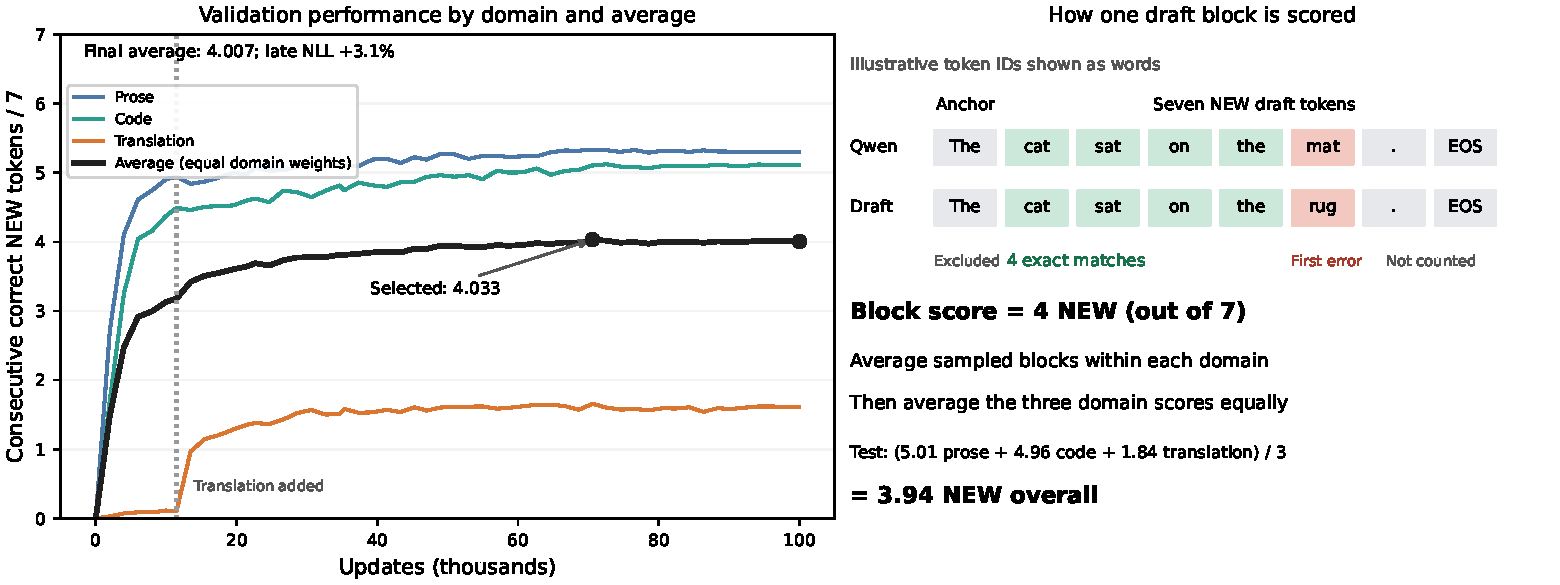
\includegraphics[width=\linewidth]{drafter-learnings-charts.pdf}

{\footnotesize \textbf{Reading the charts.} The performance curve uses held-out teacher trajectories; live verified rollouts are measured separately. The scoring example is illustrative. Domain scores average sampled blocks (up to eight per prompt); the overall score weights domains equally. One seed; matching Qwen is not human answer quality.\par}
\vspace{1mm}
{\footnotesize \textbf{References.} \href{https://arxiv.org/abs/2602.06036}{DFlash (arXiv:2602.06036)}; \href{https://transformer-circuits.pub/2026/workspace/index.html}{Anthropic workspace / Jacobian lens}. Full reports and protocols are retained in the repository.\par}
\newpage\small

{\Large\bfseries Detailed report: model and training\par}\vspace{3mm}

\vspace{2mm}{\large\bfseries What we built\par}

A separate \textbf{79M-parameter, five-layer DFlash-style drafter} learns from random weights while \textbf{Qwen2.5-0.5B stays frozen}. This is training a proposal model around an existing language model, not pretraining Qwen itself. The drafter uses Qwen's tokenizer, input embeddings and vocabulary projection; those shared weights remain frozen. Its learned layers and conditioning projection are the trainable component.

Target hidden states from post-block depths \textbf{2, 7, 12, 17 and 22} are concatenated, projected and normalized into context memory. Each draft layer attends to this memory and the current block. The selected architecture uses query/key RMSNorm, rotary positions and a gated MLP. One known anchor precedes \textbf{seven masked future positions}, predicted jointly in one pass; “diffusion-style” does not imply iterative denoising in this implementation.

\vspace{2mm}{\large\bfseries How we trained it\par}

Qwen-generated continuations supply the labels. At sampled anchors, the drafter sees only eligible pre-anchor target features and an isolated masked block. Cross-entropy supervises the seven new tokens, with exponential position weighting (gamma 4); the supplied anchor is excluded. Causal memory masks prevent future-label leakage. The final runs extract teacher features online while keeping the target frozen.

Two fresh models compared \textbf{64-token and 256-token teacher-response caps}. Both began with \textbf{131,072 prose/code examples} (65,536 per domain), then added translation to reach \textbf{196,608 balanced examples}. The transition preserved each model's optimizer, RNG and global schedule. It occurred at update 17,985 for the short arm and 11,472 for the long arm, so this comparison also changes domain-exposure timing.

Each arm completed \textbf{100,000 updates} and \textbf{268.8M supervised new-token exposures}: batch 48, eight anchors per response and seven labels per anchor. AdamW used learning rate 0.0006, weight decay 0.01, 4\% warmup, cosine scheduling and gradient clipping at 1. Seed was 42. These are token exposures with repeated sampling, not 268.8M unique tokens. Bounded Modal workers checkpointed and resumed the global run.

\vspace{2mm}{\large\bfseries How we added it to generation\par}

\textbf{1. Prefill:} Qwen processes the prompt, supplies its greedy next token as the anchor, and provides hidden-state memory. \textbf{2. Propose:} the drafter predicts up to seven following tokens in parallel. \textbf{3. Verify:} Qwen processes the proposed block; accept only the consecutive matching prefix. \textbf{4. Continue:} emit the anchor plus accepted proposals, discard rejected cache positions, append committed target features, and use Qwen's correction as the next anchor.

This is a \textbf{greedy verified decoding path}, not a standalone replacement for Qwen. The longer parity checks use FP32 verification on stored BF16 target weights. The Qwen3.5 hybrid-cache rollback path remains unimplemented. No deployment into the custom Apple inference runtime is claimed.

\newpage\small

{\Large\bfseries Detailed report: evidence and lessons\par}\vspace{3mm}

\vspace{2mm}{\large\bfseries What changed performance\par}

Early matched comparisons moved validation consecutive matches from \textbf{0.384 to 0.484} with query/key normalization, then to \textbf{0.520} with five draft layers. Five target feature depths reached \textbf{0.530}, with uncertain incremental benefit. Larger response pools and longer teacher continuations then produced the biggest improvements. These are separate studies, not one controlled cumulative attribution of the final gain.

On the same 49K examples at 6K updates, changing response caps from 64 to 256 improved long-context validation from \textbf{1.76 to 2.96}. In the final curriculum, selected short/long scores were \textbf{2.195 and 4.033 new tokens out of seven}. Keep the long-response checkpoint at \textbf{update 70,585}, not the final weights: by update 100,000, matches declined slightly to 4.007 and NLL rose from 2.105 to 2.171.

\vspace{2mm}{\large\bfseries Held-out qualification\par}

The selected long-response checkpoint was frozen before opening the test. On \textbf{189 usable prompts}, evenly split across prose, code and translation, consecutive-match scores were \textbf{5.014 / 4.958 / 1.843}, for an equal-domain average of \textbf{3.938 out of seven}. The conditional 95\% bootstrap interval for that average was \textbf{3.764--4.106}. This passes the predeclared threshold of average at least two and every domain at least one.

All \textbf{24 longer verified rollouts}, totaling \textbf{3,906 generated tokens}, matched ordinary greedy Qwen output exactly. Actual accepted new draft tokens per verification call were \textbf{4.514 prose / 4.300 code / 1.195 translation}. These live-rollout measurements use different prompts and arithmetic from cached teacher-trajectory scoring; the two metrics are not interchangeable. The chart's anchor is never counted, nor are tokens after the first mismatch.

\vspace{2mm}{\large\bfseries What we learned, and what did not work\par}

Tiny training pools could be memorized while held-out drafting stayed poor. More examples and longer responses improved generalization, but did not remove late overfitting. The training diagnostic sampled only twelve responses; it is not a full-corpus generalization-gap estimate. Earlier weak-decoder studies found no consistent gain from dropout/null-memory controls, probe-selected layers or compressed Jacobian-lens conditioning.

A separate Qwen3.5-2B target comparison remained weak (0.170 versus 0.387 new matches for the small-target comparison on shared validation sources). Target family, tokenizer, formatting and draft capacity also changed, so this does not show that larger targets inherently draft worse.

\vspace{2mm}{\large\bfseries Limits and next work\par}

These are \textbf{one-seed target-imitation results}, not evidence of human answer quality or a general wall-clock speedup. Repetitive teacher outputs, adaptive validation selection and changing curriculum/exposure limit causal claims. The drafting test is now consumed and cannot select later variants. The trained drafter does not establish from-scratch language-model capability in the separate training project.

The next J-space study is an \textbf{unfinished follow-up}: add sparse semantic conditioning alongside existing raw hidden states, with raw-only and random-frame controls and fresh held-out evaluation. Training-only helpers exist, but no new J-space fit, unverified two/three-token generation benchmark or resulting quality improvement is established. Preserve the qualified baseline while testing those hypotheses.

\vspace{2mm}{\large\bfseries Evidence and reproducibility\par}

The repository retains the full curriculum report, qualification findings, frozen checkpoint manifest, final model configuration, and executable training/decoding code. The selected checkpoint is best.pt in the fresh-grid-196608-r256-11 Modal run; its full checksum and evaluation identities are retained in the frozen manifest. No new training was run to prepare this report.
\end{document}
